% ============================================================
% Anemal SaaS — Comprehensive Functional Specification
% Version: 2.0 | Date: 2026-06-05
% Compile with: xelatex vetcare_functional_spec.tex (run twice)
% Or: pdflatex vetcare_functional_spec.tex (fallback, requires T1 fonts)
% ============================================================
\documentclass[12pt,a4paper]{report}

% ── Packages ──────────────────────────────────────────────
\usepackage[T1]{fontenc}
\usepackage[utf8]{inputenc}
\usepackage{lmodern}
\usepackage[a4paper, top=25mm, bottom=25mm, left=25mm, right=20mm, headheight=14pt]{geometry}
\usepackage{xcolor}
\usepackage[colorlinks=true,linkcolor=brandblue,urlcolor=accent,citecolor=sagegreen,
            pdftitle={Anemal SaaS Functional Specification v2.0},
            bookmarksnumbered,bookmarksopen]{hyperref}
\usepackage{titlesec}
\usepackage{tocloft}
\usepackage{enumitem}
\usepackage{longtable}
\usepackage{booktabs}
\usepackage{array}
\usepackage{tabularx}
\usepackage{fancyhdr}
\usepackage[framemethod=default]{mdframed}
\usepackage{graphicx}
\usepackage{float}
\usepackage{tikz}
\usepackage{multicol}
\usepackage{parskip}
\usepackage{microtype}
\usepackage{listings}
\usepackage{pifont}
\usepackage{amssymb}
\usepackage{amsmath}
\usetikzlibrary{shapes.geometric, arrows.meta, positioning, calc, fit, backgrounds}

% ── Colors ────────────────────────────────────────────────
\definecolor{brandblue}{HTML}{0369a1}
\definecolor{branddark}{HTML}{075985}
\definecolor{brandlight}{HTML}{e0f2fe}
\definecolor{sagegreen}{HTML}{006c4a}
\definecolor{sagelight}{HTML}{d1fae5}
\definecolor{accent}{HTML}{0ea5e9}
\definecolor{errorred}{HTML}{dc2626}
\definecolor{warnorange}{HTML}{d97706}
\definecolor{successgreen}{HTML}{16a34a}
\definecolor{codebg}{HTML}{1e293b}
\definecolor{muted}{HTML}{64748b}
\definecolor{border}{HTML}{e2e8f0}

% ── Page Setup ────────────────────────────────────────────
\pagestyle{fancy}
\fancyhf{}
\fancyhead[L]{\small\color{muted}Anemal SaaS --- Functional Specification v2.0}
\fancyhead[R]{\small\color{muted}2026-06-05}
\fancyfoot[C]{\small\color{muted}\thepage}
\renewcommand{\headrulewidth}{0.4pt}

% ── Section Styling ───────────────────────────────────────
\titleformat{\chapter}[block]
  {\normalfont\huge\bfseries\color{branddark}}{\thechapter.}{12pt}{}
  [\vspace{2pt}\color{brandlight}\rule{\linewidth}{2pt}]
\titleformat{\section}{\normalfont\large\bfseries\color{brandblue}}{\thesection}{8pt}{}
\titleformat{\subsection}{\normalfont\normalsize\bfseries\color{sagegreen}}{\thesubsection}{8pt}{}
\titleformat{\subsubsection}{\normalfont\normalsize\bfseries\color{branddark}}{\thesubsubsection}{6pt}{}

% ── Frames ────────────────────────────────────────────────
\mdfdefinestyle{InfoBox}{backgroundcolor=brandlight,linecolor=accent,linewidth=4pt,
  topline=false,bottomline=false,rightline=false,leftline=true,
  innerleftmargin=14pt,innerrightmargin=14pt,innertopmargin=10pt,innerbottommargin=10pt}
\mdfdefinestyle{SuccessBox}{backgroundcolor=sagelight,linecolor=successgreen,linewidth=4pt,
  topline=false,bottomline=false,rightline=false,leftline=true,
  innerleftmargin=14pt,innerrightmargin=14pt,innertopmargin=10pt,innerbottommargin=10pt}
\mdfdefinestyle{WarnBox}{backgroundcolor=yellow!10,linecolor=warnorange,linewidth=4pt,
  topline=false,bottomline=false,rightline=false,leftline=true,
  innerleftmargin=14pt,innerrightmargin=14pt,innertopmargin=10pt,innerbottommargin=10pt}
\mdfdefinestyle{ErrorBox}{backgroundcolor=red!5,linecolor=errorred,linewidth=4pt,
  topline=false,bottomline=false,rightline=false,leftline=true,
  innerleftmargin=14pt,innerrightmargin=14pt,innertopmargin=10pt,innerbottommargin=10pt}

% ── Code ──────────────────────────────────────────────────
\lstset{basicstyle=\ttfamily\small,backgroundcolor=\color{codebg},
  keywordstyle=\color{accent}\bfseries,commentstyle=\color{muted},
  stringstyle=\color{successgreen},numberstyle=\tiny\color{muted},
  numbers=left,stepnumber=1,numbersep=8pt,frame=none,
  breaklines=true,showstringspaces=false,xleftmargin=16pt,tabsize=2}

% ── Custom Commands ───────────────────────────────────────
\newcommand{\must}{\colorbox{red!15}{\color{errorred}\textbf{\small MUST}}}
\newcommand{\should}{\colorbox{orange!15}{\color{warnorange}\textbf{\small SHOULD}}}
\newcommand{\could}{\colorbox{green!10}{\color{successgreen}\textbf{\small COULD}}}
\newcommand{\complete}{\textcolor{successgreen}{\ding{51}~\textbf{Complete}}}
\newcommand{\planned}{\textcolor{warnorange}{$\circ$~\textbf{Planned}}}
\newcommand{\testcheck}{\textcolor{successgreen}{\ding{51}}}
\newcommand{\testpending}{\textcolor{warnorange}{$\circ$}}
\newcommand{\moduleheader}[2]{%
  \par\vspace{6pt}%
  \noindent\colorbox{branddark}{\color{white}\textbf{\small #1}}\quad\textbf{\large #2}%
  \par\vspace{4pt}%
}

% ── Table column types ────────────────────────────────────
\renewcommand{\arraystretch}{1.35}
\newcolumntype{L}[1]{>{\raggedright\arraybackslash}p{#1}}
\newcolumntype{C}[1]{>{\centering\arraybackslash}p{#1}}

% ============================================================
\begin{document}

% ── Cover Page ────────────────────────────────────────────
\begin{titlepage}
\pagecolor{branddark}\color{white}
\vspace*{36mm}
\begin{center}
  {\fontsize{40}{46}\selectfont\bfseries Anemal SaaS}\\[5mm]
  {\fontsize{20}{26}\selectfont Comprehensive Functional Specification}\\[4mm]
  {\color{brandlight}\rule{110mm}{1.5pt}}\\[6mm]
  {\large Multi-Tenant Veterinary Clinic Management Platform}\\[12mm]
  \begin{tabular}{rl}
    \textbf{Version:}      & 2.0 \\[2pt]
    \textbf{Date:}         & 2026-06-05 \\[2pt]
    \textbf{Status:}       & Phase 1--3 Complete, Phase 4 Planned \\[2pt]
    \textbf{Modules:}      & 13 Functional + Architecture + Infrastructure \\[2pt]
    \textbf{DB Tables:}    & 25 tables, PostgreSQL 15+ with RLS \\[2pt]
    \textbf{Platforms:}    & Web Browser + Tablet (Touch-first) \\
  \end{tabular}\\[14mm]
  {\color{muted}\small Compiled: \today}
\end{center}
\end{titlepage}
\pagecolor{white}\color{black}
\setcounter{tocdepth}{2}
\tableofcontents
\clearpage

% ============================================================
\chapter{Introduction \& System Overview}

\section{Product Description}

Anemal SaaS is a \textbf{multi-tenant Software-as-a-Service} platform for veterinary clinics. It supports both \textbf{Web Browser} (reception counter, 1024px+) and \textbf{Tablet} (touch-first, consultation room, min tap target 44x44px) clients, with full multi-branch capability under a single subscription.

\begin{mdframed}[style=InfoBox]
\textbf{Multi-Tenancy Model:} Shared database, shared schema. Every tenant-scoped table carries \texttt{tenant\_id}. PostgreSQL Row-Level Security (RLS) enforces hard data isolation between clinics at the database layer --- even if application code has a bug.
\end{mdframed}

\section{User Roles}

\begin{longtable}{L{2.5cm} L{3.5cm} L{8cm}}
\toprule
\textbf{Role} & \textbf{Title} & \textbf{Access Scope} \\\midrule\endhead\bottomrule\endfoot
\texttt{admin}      & Clinic Owner / Manager     & Full access within tenant: users, branches, reports, all settings \\
\texttt{doctor}     & Veterinarian               & EMR, Inpatient, Blood Bank, Appointments, Prescriptions \\
\texttt{staff}      & Assistant / Counter / Groomer & Grooming, Appointments, Billing/POS, Pet Profiles, Retail POS \\
\texttt{superadmin} & Platform Operator          & Cross-tenant: tenant management, subscriptions, platform health \\
\end{longtable}

\section{Subscription Plans}

\begin{longtable}{L{3cm} L{2.5cm} L{2.5cm} L{5.5cm}}
\toprule
\textbf{Plan} & \textbf{Branches} & \textbf{Users} & \textbf{Included Modules} \\\midrule\endhead\bottomrule\endfoot
\texttt{starter}       & 1        & Up to 5   & Auth, Pets, Appointments, EMR, Billing \\
\texttt{professional}  & Up to 3  & Up to 15  & Starter + Inventory, Reports, Loyalty \\
\texttt{clinic\_plus}  & Unlimited & Unlimited & All modules: Inpatient, Grooming, Blood Bank \\
\end{longtable}

\section{Development Phases}

\begin{longtable}{C{1.5cm} L{4cm} L{6cm} C{2.5cm}}
\toprule
\textbf{Phase} & \textbf{Focus} & \textbf{Key Deliverables} & \textbf{Status} \\\midrule\endhead\bottomrule\endfoot
1 & Foundation \& Security  & Auth, Multi-tenancy, Base UI, Dashboard  & \complete \\
2 & Core Clinic Operations  & Pet/Owner, Appointments, EMR, Prescriptions & \complete \\
3 & Commercial Operations   & Inventory, Billing/POS, Reports, SaaS Plans & \complete \\
4 & Advanced \& Scaling     & Inpatient, Grooming, Blood Bank, Loyalty  & \planned \\
\end{longtable}

% ============================================================
\chapter{System Architecture}

\section{Architecture Overview}

Anemal uses a \textbf{layered monolith with service boundaries} architecture, optimised for rapid feature delivery while keeping multi-tenant isolation guarantees firm.

\begin{figure}[H]
\centering
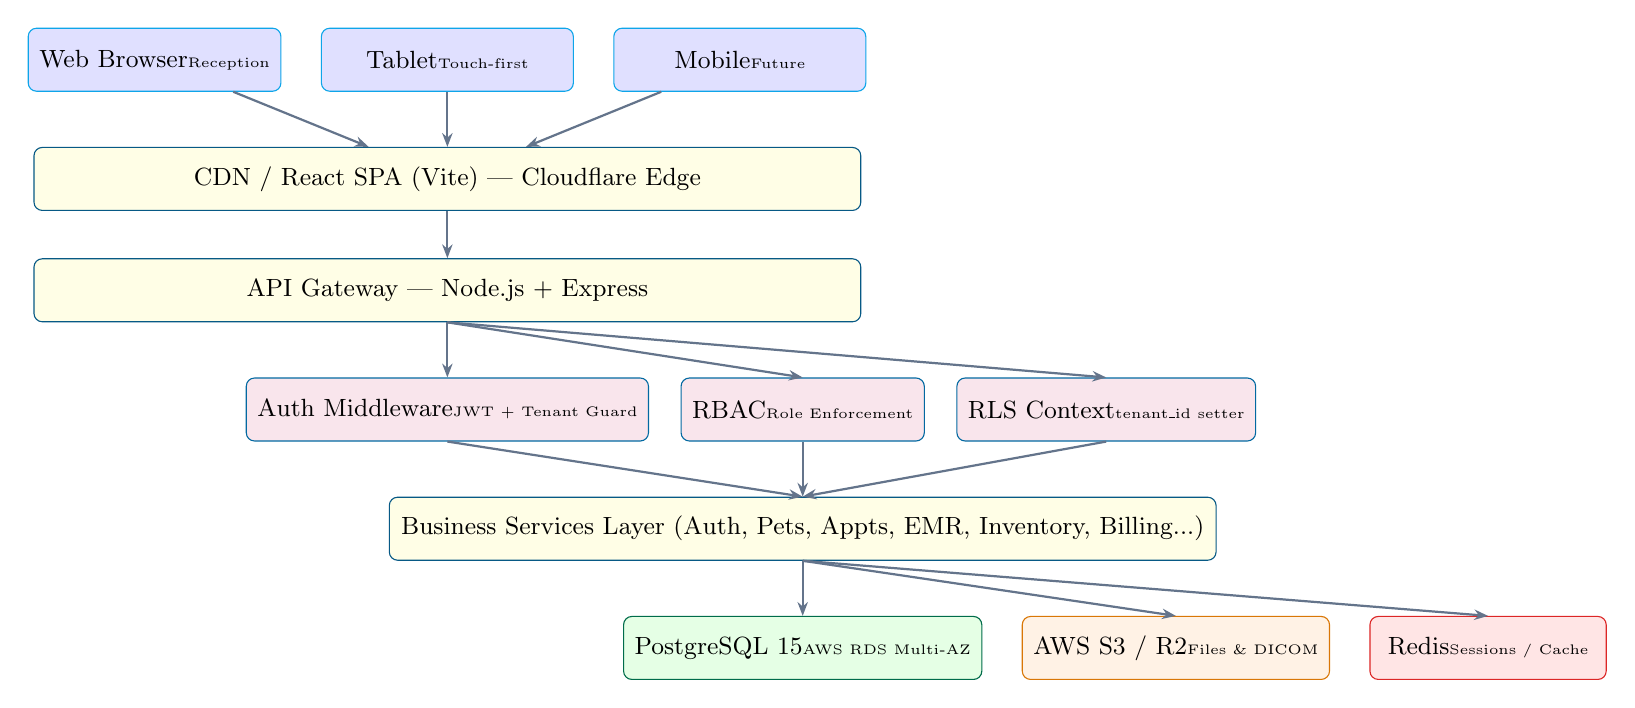
\begin{tikzpicture}[
  box/.style={rectangle,draw,rounded corners=3pt,minimum width=3.2cm,minimum height=0.8cm,font=\small,text centered,inner sep=4pt},
  client/.style={box,fill=blue!12,draw=accent},
  mid/.style={box,fill=yellow!10,draw=branddark},
  mw/.style={box,fill=purple!10,draw=brandblue},
  db/.style={box,fill=green!10,draw=sagegreen},
  store/.style={box,fill=orange!10,draw=warnorange},
  cache/.style={box,fill=red!10,draw=errorred},
  arr/.style={-{Stealth[length=5pt]},thick,color=muted}
]
\node[client] (web) {Web Browser\\{\tiny Reception}};
\node[client, right=0.5cm of web] (tab) {Tablet\\{\tiny Touch-first}};
\node[client, right=0.5cm of tab] (mob) {Mobile\\{\tiny Future}};
\node[mid, below=0.7cm of tab, minimum width=10.5cm] (spa) {CDN / React SPA (Vite) --- Cloudflare Edge};
\node[mid, below=0.6cm of spa, minimum width=10.5cm] (api) {API Gateway --- Node.js + Express};
\node[mw, below=0.7cm of api, minimum width=3cm] (am) {Auth Middleware\\{\tiny JWT + Tenant Guard}};
\node[mw, right=0.4cm of am, minimum width=3cm] (rb) {RBAC\\{\tiny Role Enforcement}};
\node[mw, right=0.4cm of rb, minimum width=3cm] (rls) {RLS Context\\{\tiny tenant\_id setter}};
\node[mid, below=0.7cm of rb, minimum width=10.5cm] (svc) {Business Services Layer (Auth, Pets, Appts, EMR, Inventory, Billing...)};
\node[db, below=0.7cm of svc, minimum width=3cm] (pg) {PostgreSQL 15\\{\tiny AWS RDS Multi-AZ}};
\node[store, right=0.5cm of pg, minimum width=3cm] (s3) {AWS S3 / R2\\{\tiny Files \& DICOM}};
\node[cache, right=0.5cm of s3, minimum width=3cm] (rd) {Redis\\{\tiny Sessions / Cache}};
\draw[arr] (web) -- (spa); \draw[arr] (tab) -- (spa); \draw[arr] (mob) -- (spa);
\draw[arr] (spa) -- (api);
\draw[arr] (api.south) -- (am.north);
\draw[arr] (api.south) -- (rb.north);
\draw[arr] (api.south) -- (rls.north);
\draw[arr] (am.south) -- (svc.north);
\draw[arr] (rb.south) -- (svc.north);
\draw[arr] (rls.south) -- (svc.north);
\draw[arr] (svc.south) -- (pg.north);
\draw[arr] (svc.south) -- (s3.north);
\draw[arr] (svc.south) -- (rd.north);
\end{tikzpicture}
\caption{Anemal SaaS System Architecture}
\end{figure}

\section{Layered Architecture Pattern}

Every API request follows \textbf{Route \textrightarrow{} Controller \textrightarrow{} Service \textrightarrow{} Repository}:

\begin{enumerate}
  \item \textbf{Route:} HTTP method, path, middleware chain. Zero business logic.
  \item \textbf{Controller:} Input validation (Zod schema), call service, format HTTP response.
  \item \textbf{Service:} All business logic. Receives \texttt{tenantId} as explicit parameter.
  \item \textbf{Repository:} Database queries only. Always scoped to \texttt{tenant\_id} (and \texttt{branch\_id} where applicable).
\end{enumerate}

\begin{mdframed}[style=ErrorBox]
\textbf{Critical Security Rule:} Every SELECT / INSERT / UPDATE / DELETE on tenant-scoped tables MUST include \texttt{WHERE tenant\_id = :currentTenantId}. Enforced additionally by PostgreSQL RLS. Any violation is a \textbf{Critical Security Bug} and must be rejected in code review.
\end{mdframed}

\section{Frontend Stack}

\begin{longtable}{L{3.5cm} L{10cm}}
\toprule
\textbf{Technology} & \textbf{Purpose} \\\midrule\endhead\bottomrule\endfoot
React 18            & SPA with concurrent rendering for smooth tablet UX \\
TypeScript (strict) & Eliminates undefined-behaviour in critical medical data paths \\
Vite                & Sub-second HMR; optimised production bundles \\
Tailwind CSS        & Utility-first; design tokens (Compassionate Care System) in \texttt{tailwind.config.js} \\
React Query         & Server state; automatic cache invalidation and background refresh \\
Zustand             & Local state: auth, sidebar toggle, active branch context \\
React Router v6     & SPA routing; \texttt{ProtectedRoute} wrapper for authentication \\
Material Symbols Outlined & Icon system via Google Fonts CDN --- no emoji in navigation \\
\end{longtable}

\section{Backend Stack}

\begin{longtable}{L{3.5cm} L{10cm}}
\toprule
\textbf{Technology} & \textbf{Purpose} \\\midrule\endhead\bottomrule\endfoot
Node.js 20 LTS  & Non-blocking I/O for concurrent clinic traffic \\
Express 5       & Minimal HTTP framework; middleware pipeline \\
Prisma ORM      & Type-safe DB client; middleware injects \texttt{tenant\_id} into every query automatically \\
PostgreSQL 15   & Primary DB; JSONB, RLS, index-only scans for multi-tenant performance \\
Redis           & Token blacklist (logout), rate-limit state, session cache \\
Zod             & Runtime input validation on all API endpoints \\
bcrypt (cost=12) & Password hashing \\
jsonwebtoken    & JWT signing RS256 (asymmetric keys) \\
\end{longtable}

% ============================================================
\chapter{Infrastructure \& DevOps}

\section{Cloud Infrastructure (AWS)}

\begin{longtable}{L{3.5cm} L{4.5cm} L{6cm}}
\toprule
\textbf{Component} & \textbf{AWS Service} & \textbf{Configuration} \\\midrule\endhead\bottomrule\endfoot
API Servers      & EC2 + Auto Scaling   & t3.medium; min 2 / max 10 instances; ap-southeast-1a/b \\
Database         & RDS PostgreSQL 15    & db.t3.large; Multi-AZ; 30-day automated backups \\
File Storage     & S3 + CloudFront      & SSE-S3 encryption; pre-signed URLs for DICOM \\
Cache/Sessions   & ElastiCache Redis 7  & cache.t3.micro; cluster mode; TLS \\
CDN/Static       & CloudFront           & React SPA dist; HTTPS enforced; edge caching \\
Load Balancer    & ALB                  & SSL termination; /api/health checks; sticky sessions off \\
DNS              & Route 53             & Wildcard \texttt{*.anemal.app} to ALB \\
Secrets          & AWS Secrets Manager  & DB creds, JWT private keys, API keys \\
Monitoring       & CloudWatch + Grafana & API latency, DB connections, error rates \\
Alerting         & PagerDuty + SNS      & P1: 2-min SLA; P2: 15-min SLA \\
\end{longtable}

\section{Multi-Tenancy Subdomain Routing}

\begin{enumerate}
  \item DNS wildcard \texttt{*.anemal.app} resolves to ALB.
  \item ALB forwards to Express API cluster.
  \item \textbf{Tenant Resolver Middleware} reads \texttt{Host} header, extracts subdomain, queries \texttt{tenants} table.
  \item \texttt{tenant\_id} injected into request context.
  \item Prisma middleware: before every query, executes \texttt{SET app.current\_tenant\_id = \$tenantId}.
  \item PostgreSQL RLS policies fire automatically using this session variable.
\end{enumerate}

\section{CI/CD Pipeline}

\begin{longtable}{L{3cm} L{4cm} L{7cm}}
\toprule
\textbf{Stage} & \textbf{Tool} & \textbf{Actions} \\\midrule\endhead\bottomrule\endfoot
Code Quality     & ESLint + tsc strict    & Lint, type-check, import ordering \\
Unit Tests       & Jest                   & Services, controllers, hooks ($>$80\% coverage) \\
Integration Tests & Supertest + test DB   & Full API endpoint + cross-tenant isolation tests \\
Security Scan    & npm audit + Snyk       & Dependency vulnerability check \\
Build            & Vite + tsc             & Production bundle + type compile \\
Container Build  & Docker + ECR           & Multi-stage Dockerfile; image vulnerability scan \\
Deploy Staging   & ECS Fargate            & Auto-deploy on \texttt{main} branch push \\
Deploy Prod      & ECS Fargate Blue/Green & Manual approval gate; zero-downtime swap \\
\end{longtable}

\section{Backup \& Disaster Recovery}

\begin{itemize}
  \item \textbf{Database:} RDS automated daily snapshots; 30-day retention; PITR to any second.
  \item \textbf{Files:} S3 versioning enabled; cross-region replication to \texttt{ap-southeast-2}.
  \item \textbf{RTO:} 4 hours. \textbf{RPO:} 1 hour.
\end{itemize}

% ============================================================
\chapter{Application Management (SaaS Platform Level)}

\section{Description}

Application Management covers the \textbf{SaaS platform operator} layer --- tools used by the Anemal engineering/operations team to manage the platform itself. This is \emph{separate} from the admin panel available to clinic owners.

\section{Super Admin Portal (\texttt{/superadmin})}

Accessible only to \texttt{superadmin} role. Protected by TOTP MFA (mandatory).

\subsection{Tenant Management}

\begin{longtable}{L{4cm} L{10cm}}
\toprule
\textbf{Function} & \textbf{Description} \\\midrule\endhead\bottomrule\endfoot
List All Tenants   & Paginated: name, subdomain, plan, status, created, last active \\
View Tenant Detail & User count, branch count, monthly revenue, storage usage \\
Suspend Tenant     & \texttt{tenants.is\_active = false}; all logins return 403 with suspension message \\
Reactivate Tenant  & Restores access; notifies tenant admin \\
Delete Tenant      & Soft delete; 30-day GDPR-compliant data retention before purge \\
Impersonate        & Log in as tenant admin for support (audit-logged as \texttt{superadmin\_impersonate}) \\
\end{longtable}

\subsection{Subscription Management}

\begin{longtable}{L{4cm} L{10cm}}
\toprule
\textbf{Function} & \textbf{Description} \\\midrule\endhead\bottomrule\endfoot
Plan Assignment    & Change tenant plan with immediate effect \\
Trial Management   & Extend/view trial; send upgrade reminders \\
Invoice Generation & Monthly SaaS subscription invoices via email \\
Payment Integration & Omise recurring billing for subscription fees \\
Revenue Dashboard  & MRR, ARR, churn rate, new signups charts \\
\end{longtable}

\section{Tenant Onboarding Workflow}

\begin{enumerate}
  \item Clinic owner visits \texttt{anemal.app/register}: submits clinic name, subdomain, admin email, password, phone.
  \item System validates subdomain uniqueness; returns \texttt{409 Conflict} if taken.
  \item \textbf{Atomic transaction:} creates \texttt{tenants} + default \texttt{branches} + first \texttt{users} (admin) record.
  \item \texttt{trial\_ends\_at = NOW() + 30 days} set.
  \item Welcome email (SendGrid) sent with login link and setup guide.
  \item Tenant admin configures: logo, address, operating hours, doctor shifts, initial inventory.
  \item Trial-to-paid: admin selects plan and enters payment via Omise.
\end{enumerate}

\section{Testing Criteria}

\begin{itemize}
  \item[\testcheck] Registration: all 3 records created atomically; any failure rolls back completely.
  \item[\testcheck] Subdomain duplicate: \texttt{409} without leaking other tenant names.
  \item[\testcheck] Suspended tenant: all API calls return \texttt{403}.
  \item[\testcheck] Impersonation logged in \texttt{audit\_logs} with \texttt{superadmin\_impersonate} action.
  \item[\testcheck] Plan downgrade blocked if tenant exceeds new plan's branch/user limits.
  \item[\testpending] Trial expiry cron: auto-suspend at midnight UTC on expiry date.
  \item[\testpending] GDPR delete purge runs 30 days after soft delete.
\end{itemize}

% ============================================================
\chapter{FR-01: Authentication \& Authorization}

\moduleheader{FR-01}{Authentication \& Authorization}

\section{Description}

Secure identity verification and role-based access control using JWT (RS256), bcrypt password hashing, sliding refresh-token mechanism optimised for an 8-hour clinical workday, and per-user time-window access restrictions.

\section{Prerequisites}

\begin{itemize}
  \item \texttt{users} table with \texttt{tenant\_id}, \texttt{role}, \texttt{password\_hash}, \texttt{is\_active}, \texttt{allowed\_start\_time}, \texttt{allowed\_end\_time}.
  \item Redis instance for token blacklisting and rate-limit state.
  \item \texttt{JWT\_ACCESS\_SECRET} and \texttt{JWT\_REFRESH\_SECRET} in AWS Secrets Manager.
  \item Subdomain-to-tenant resolver middleware deployed upstream.
\end{itemize}

\section{Process Flow}

\begin{enumerate}
  \item User navigates to \texttt{https://[subdomain].anemal.app}.
  \item Frontend calls \texttt{GET /api/tenant/resolve} to confirm tenant context.
  \item User submits email + password.
  \item \textbf{Rate limit check:} 5 failed attempts per email per 15 min (Redis); exceed: \texttt{429}.
  \item Server: find user by \texttt{(tenant\_id, email)} \textrightarrow{} verify bcrypt hash.
  \item \textbf{Time window check:} if \texttt{allowed\_start\_time / allowed\_end\_time} configured, verify current time.
  \item On success: generate \textbf{Access Token} (8h, RS256) + \textbf{Refresh Token} (30d, \texttt{HttpOnly} cookie).
  \item JWT payload: \texttt{\{userId, tenantId, branchId, role, iat, exp\}}.
  \item All API requests: \texttt{Authorization: Bearer <accessToken>}.
  \item Auth Middleware validates token \textrightarrow{} sets \texttt{app.current\_tenant\_id} PostgreSQL session variable.
  \item RBAC Middleware: \texttt{requireRole(...)} checks \texttt{role} claim.
  \item Token refresh: \texttt{POST /api/auth/refresh} \textrightarrow{} validate cookie \textrightarrow{} issue new access token.
  \item Logout: \texttt{POST /api/auth/logout} \textrightarrow{} blacklist refresh token in Redis.
\end{enumerate}

\section{API Endpoints}

\begin{longtable}{L{1.5cm} L{5cm} L{7.5cm}}
\toprule
\textbf{Method} & \textbf{Endpoint} & \textbf{Description} \\\midrule\endhead\bottomrule\endfoot
POST   & \texttt{/api/auth/login}     & Login; returns access token + sets refresh cookie \\
POST   & \texttt{/api/auth/refresh}   & Refresh access token using cookie \\
POST   & \texttt{/api/auth/logout}    & Invalidate refresh token \\
GET    & \texttt{/api/auth/me}        & Current user profile \\
POST   & \texttt{/api/users}          & Create user (Admin only) \\
GET    & \texttt{/api/users}          & List users in tenant (Admin only) \\
PUT    & \texttt{/api/users/:id}      & Update user (Admin only) \\
DELETE & \texttt{/api/users/:id}      & Soft-deactivate user (Admin only) \\
\end{longtable}

\section{Functional Requirements}

\begin{longtable}{L{2.5cm} L{9cm} C{2cm}}
\toprule
\textbf{ID} & \textbf{Requirement} & \textbf{Priority} \\\midrule\endhead\bottomrule\endfoot
FR-01-01 & Login with email + password & \must \\
FR-01-02 & JWT embeds \texttt{tenant\_id, branch\_id, user\_id, role} & \must \\
FR-01-03 & Access token 8h expiry; refresh token 30d & \must \\
FR-01-04 & Role-Based Access Control (Admin / Doctor / Staff) & \must \\
FR-01-05 & Admin can add/deactivate users and assign roles & \must \\
FR-01-06 & Per-user login time-window restrictions & \should \\
\end{longtable}

\section{Testing Criteria}

\begin{itemize}
  \item[\testcheck] Valid credentials: \texttt{200} with \texttt{accessToken}; \texttt{refreshToken} in \texttt{HttpOnly} cookie.
  \item[\testcheck] Wrong password: \texttt{401} --- message does NOT reveal whether email exists.
  \item[\testcheck] 5 failures in 15 min: \texttt{429} rate limit enforced.
  \item[\testcheck] JWT payload contains \texttt{tenantId}, \texttt{role}, \texttt{exp}.
  \item[\testcheck] Expired access token: \texttt{401}; refresh issues new token.
  \item[\testcheck] Reused blacklisted refresh token: rejected.
  \item[\testcheck] Staff on Admin-only endpoint: \texttt{403}.
  \item[\testcheck] Deactivated user (\texttt{is\_active = false}): cannot log in.
  \item[\testcheck] Cannot deactivate last active admin in tenant.
  \item[\testcheck] Login outside allowed time window: \texttt{403} ``Access not permitted at this time.''
\end{itemize}

% ============================================================
\chapter{FR-02: Multi-Tenancy \& Multi-Branch}

\moduleheader{FR-02}{Multi-Tenancy \& Multi-Branch Setup}

\section{Description}

Foundational isolation layer. Every clinic is completely isolated. Within a tenant, multiple branches share the same subscription but have independent inventory, schedules, and staff.

\section{Prerequisites}

\begin{itemize}
  \item PostgreSQL RLS policies enabled on all 25 tenant-scoped tables.
  \item Wildcard DNS \texttt{*.anemal.app} pointing to ALB.
  \item Tenant resolver and \texttt{app.current\_tenant\_id} setter middleware in pipeline.
\end{itemize}

\section{Tenant Isolation Process Flow}

\begin{enumerate}
  \item HTTP request arrives; \texttt{Host} header = \texttt{abc-clinic.anemal.app}.
  \item Tenant Resolver: extract \texttt{abc-clinic} \textrightarrow{} \texttt{SELECT id FROM tenants WHERE subdomain = 'abc-clinic'}.
  \item \texttt{req.tenantId} set.
  \item Prisma middleware: before every query \textrightarrow{} \texttt{SET app.current\_tenant\_id = tenantId}.
  \item PostgreSQL RLS: \texttt{USING (tenant\_id = current\_setting('app.current\_tenant\_id')::INT)} fires automatically.
  \item All queries auto-scoped. Developer mistakes (missing WHERE clause) are silently caught by RLS.
\end{enumerate}

\section{Functional Requirements}

\begin{longtable}{L{2.5cm} L{9cm} C{2cm}}
\toprule
\textbf{ID} & \textbf{Requirement} & \textbf{Priority} \\\midrule\endhead\bottomrule\endfoot
FR-02-01 & Unique subdomain per clinic & \must \\
FR-02-02 & Every table row isolated by \texttt{tenant\_id} & \must \\
FR-02-03 & No user can see any other clinic's data under any circumstances & \must \\
FR-02-04 & Multi-branch under one tenant; transactions by \texttt{branch\_id} & \must \\
FR-02-05 & Admin sets branch info, hours, address, doctor shifts per branch & \must \\
FR-02-06 & Super Admin overview of all tenants (platform level) & \should \\
\end{longtable}

\section{Testing Criteria}

\begin{itemize}
  \item[\testcheck] Tenant A user accessing Tenant B resource by guessed ID: \texttt{404} (never \texttt{403}).
  \item[\testcheck] Forged JWT with wrong \texttt{tenantId}: RLS returns empty results.
  \item[\testcheck] Cross-tenant isolation test on all 25 tables: 0 rows leaked.
  \item[\testcheck] Branch name uniqueness within tenant enforced.
  \item[\testcheck] Doctor shifts set in Branch A not visible in Branch B scheduler.
  \item[\testcheck] Subdomain duplicate on registration: \texttt{409}.
\end{itemize}

% ============================================================
\chapter{FR-03: Pet \& Owner Management (CRM)}

\moduleheader{FR-03}{Pet \& Owner Management}

\section{Description}

Core CRM of Anemal. Manages the lifecycle of pet owner profiles and their associated pets. Every medical, billing, and appointment record links back here. Supports smart onboarding, photo capture, drug allergy tracking, and proactive health reminders.

\section{Prerequisites}

\begin{itemize}
  \item User authenticated with \texttt{staff}, \texttt{doctor}, or \texttt{admin} role.
  \item S3 bucket configured for pet photo uploads.
  \item (Optional) ID card reader hardware at reception workstation.
\end{itemize}

\section{Process Flow: New Pet Registration}

\begin{enumerate}
  \item Staff Quick-Search for existing owner (by phone/name/microchip).
  \item If new: complete Owner form (or scan ID card for auto-fill of name, address, ID).
  \item System validates phone number uniqueness within tenant.
  \item Create owner: \texttt{first\_name, last\_name, phone, email, address, line\_user\_id}.
  \item Add pet(s): name, species, breed, DOB, gender, color, microchip ID.
  \item Upload pet photo from Tablet camera or file; stored in S3, URL in \texttt{pets.photo\_url}.
  \item Record drug allergies (TEXT[]) and underlying conditions.
  \item System auto-generates initial reminder schedule (vaccination, deworming) based on species and age.
\end{enumerate}

\section{Process Flow: Proactive Reminder}

\begin{enumerate}
  \item Nightly cron: query \texttt{pet\_reminders} where \texttt{due\_date = TODAY + 7} and \texttt{status = 'pending'}.
  \item Send LINE/SMS notification to owner.
  \item Update \texttt{status = 'sent'}, \texttt{sent\_at = NOW()}.
  \item Doctor/staff marks \texttt{completed} when vaccination administered.
\end{enumerate}

\section{Functional Requirements}

\begin{longtable}{L{2.5cm} L{9cm} C{2cm}}
\toprule
\textbf{ID} & \textbf{Requirement} & \textbf{Priority} \\\midrule\endhead\bottomrule\endfoot
FR-03-01 & Create/edit/deactivate owner profiles & \must \\
FR-03-02 & Smart onboarding via ID card reader & \should \\
FR-03-03 & Create/edit pet profiles (name, species, breed, DOB, sex, color, microchip) & \must \\
FR-03-04 & Drug allergy and underlying condition records; prominently shown in EMR & \must \\
FR-03-05 & Pet photo upload from Tablet camera or file & \must \\
FR-03-06 & Quick search: pet name, owner name, phone, microchip ID & \must \\
FR-03-07 & Infectious disease watch flag with reason & \should \\
FR-03-08 & Vaccination timeline on pet profile & \must \\
FR-03-09 & Proactive health reminders (vaccination, deworming) via LINE/SMS & \must \\
\end{longtable}

\section{Key Business Rules}

\begin{itemize}
  \item Drug allergies (\texttt{pets.allergies} TEXT[]) displayed in \textbf{red} in all prescription and EMR screens.
  \item Flagged pets (\texttt{is\_flagged = true}) show persistent warning badge throughout system.
  \item Deceased pets (\texttt{is\_deceased = true}) hidden from active search but preserved for history.
  \item Microchip ID unique within a tenant.
\end{itemize}

\section{Testing Criteria}

\begin{itemize}
  \item[\testcheck] Duplicate phone within tenant: \texttt{409}.
  \item[\testcheck] Pet photo uploads to S3; URL saved in DB.
  \item[\testcheck] Quick search returns results in $<$500ms for 10,000-pet tenant.
  \item[\testcheck] Drug allergy badge visible (red) in prescription screens.
  \item[\testcheck] Deceased pet excluded from appointment Quick Search.
  \item[\testcheck] Proactive reminder cron selects correct pets 7 days before due date.
  \item[\testcheck] Vaccination timeline shows all vaccines in chronological order.
\end{itemize}

% ============================================================
\chapter{FR-04: Appointment \& Scheduler}

\moduleheader{FR-04}{Appointment \& Scheduler}

\section{Description}

Manages daily clinic scheduling with weekly/daily calendar views per branch and doctor, walk-in queue, double-booking detection, and automated LINE/SMS reminders 24 hours before appointments.

\section{Prerequisites}

\begin{itemize}
  \item Doctor shifts configured per branch (\texttt{doctor\_shifts} table).
  \item Pet and owner profiles exist.
  \item LINE Messaging API credentials configured (for reminders).
  \item Branch operating hours set.
\end{itemize}

\section{Process Flow: Scheduled Appointment}

\begin{enumerate}
  \item Staff selects date/time on calendar; system shows available doctors and rooms.
  \item \textbf{Double-booking check:} query overlapping \texttt{(doctor\_id, appointment\_date, duration\_min)}.
  \item Select pet (Quick Search) \textrightarrow{} auto-fill owner info.
  \item Set reason, room, duration (default 30 min). Save \textrightarrow{} \texttt{status = 'scheduled'}.
  \item LINE confirmation sent to owner.
  \item 24h before: cron sends LINE/SMS reminder; \texttt{reminder\_sent\_at} updated.
  \item Day of: status progression: \texttt{scheduled} \textrightarrow{} \texttt{confirmed} \textrightarrow{} \texttt{in\_progress} \textrightarrow{} \texttt{completed}.
  \item On \texttt{completed}: system prompts to create EMR.
\end{enumerate}

\section{Process Flow: Walk-in Queue}

\begin{enumerate}
  \item Staff clicks ``Walk-in'' on Queue panel.
  \item Quick-search pet (or create new on spot).
  \item Appointment: \texttt{is\_walk\_in = true}, \texttt{status = 'in\_progress'}, \texttt{appointment\_date = NOW()}.
  \item Pet appears in Today's Queue; doctor begins consultation.
\end{enumerate}

\section{Appointment Status Lifecycle}

\begin{longtable}{L{3.5cm} L{10.5cm}}
\toprule
\textbf{Status} & \textbf{Meaning} \\\midrule\endhead\bottomrule\endfoot
\texttt{scheduled}    & Appointment booked; not confirmed by client \\
\texttt{confirmed}    & Client confirmed (reminder reply or phone call) \\
\texttt{in\_progress} & Pet currently being examined \\
\texttt{completed}    & Consultation finished; links to medical record \\
\texttt{cancelled}    & Cancelled with optional reason \\
\texttt{no\_show}     & Client did not appear without cancelling \\
\end{longtable}

\section{Functional Requirements}

\begin{longtable}{L{2.5cm} L{9cm} C{2cm}}
\toprule
\textbf{ID} & \textbf{Requirement} & \textbf{Priority} \\\midrule\endhead\bottomrule\endfoot
FR-04-01 & Weekly/Daily calendar per branch & \must \\
FR-04-02 & Filter by doctor, room, type & \must \\
FR-04-03 & 6-status appointment lifecycle & \must \\
FR-04-04 & LINE/SMS reminder 24h in advance & \should \\
FR-04-05 & Doctor's Today Schedule on Tablet & \must \\
FR-04-06 & Double-booking detection and blocking & \must \\
FR-04-07 & Walk-in queue without pre-booking & \must \\
\end{longtable}

\section{Testing Criteria}

\begin{itemize}
  \item[\testcheck] Same doctor/room overlapping time: \texttt{409 Conflict}.
  \item[\testcheck] Walk-in: \texttt{is\_walk\_in = true}, \texttt{status = 'in\_progress'}.
  \item[\testcheck] Calendar renders all branch appointments in date range correctly.
  \item[\testcheck] Reminder cron: 24h ahead appointments selected; LINE sent; \texttt{reminder\_sent\_at} updated.
  \item[\testcheck] Invalid status transitions (e.g., \texttt{completed} \textrightarrow{} \texttt{scheduled}) rejected.
  \item[\testcheck] Appointment outside branch operating hours generates warning.
\end{itemize}

% ============================================================
\chapter{FR-05: Electronic Medical Record (EMR)}

\moduleheader{FR-05}{Electronic Medical Record \& Clinical}

\section{Description}

Clinical heart of Anemal. Records consultations in SOAP format, captures vital signs via touch-friendly steppers, manages prescriptions linked to live inventory, supports lab results with trend graphs, DICOM image viewing, anatomy annotation canvas (Konva.js with Stylus/Touch), and PDF export for referrals.

\section{Prerequisites}

\begin{itemize}
  \item Appointment with status \texttt{in\_progress} (or direct doctor creation).
  \item Pet drug allergy list loaded and displayed.
  \item Branch inventory active (for real-time prescription stock check).
  \item S3 bucket for lab result files and DICOM images.
\end{itemize}

\section{Process Flow: Clinical Consultation}

\begin{enumerate}
  \item Doctor opens appointment \textrightarrow{} ``Start Consultation'' \textrightarrow{} creates \texttt{medical\_records} row.
  \item \textbf{Drug Allergy Alert:} if \texttt{pets.allergies} non-empty, red alert banner shown at page top.
  \item Enter \textbf{SOAP Note:}
    \begin{itemize}
      \item \textbf{S (Subjective):} Chief complaint, owner-reported history.
      \item \textbf{O (Objective):} Physical exam, lab findings.
      \item \textbf{A (Assessment):} Diagnosis / differential diagnosis.
      \item \textbf{P (Plan):} Treatment plan, follow-up instructions.
    \end{itemize}
  \item Record \textbf{Vital Signs} via touch steppers: weight (kg), temperature ($^\circ$C), heart rate (bpm), resp. rate (rpm).
  \item \textbf{Prescription:} search drug \textrightarrow{} check real-time branch stock \textrightarrow{} check against allergies \textrightarrow{} set dosage + duration \textrightarrow{} save \textrightarrow{} stock auto-deducted.
  \item \textbf{Lab Tests:} order tests; enter numeric structured results with units; upload PDF summary. Plot trend graph with $\geq$2 data points.
  \item \textbf{Anatomy Annotation:} select species template; draw on Konva.js canvas with Stylus/finger; save as JSONB.
  \item Attach X-ray/ultrasound DICOM images; view via Cornerstone.js embedded viewer.
  \item Doctor marks record \texttt{completed} \textrightarrow{} triggers billing draft invoice.
\end{enumerate}

\begin{mdframed}[style=ErrorBox]
\textbf{Prescription Safety Rules} (must both pass before saving):
\begin{enumerate}
  \item Drug allergy match: \textbf{hard block} --- requires explicit doctor override confirmation. Not just a warning.
  \item Zero stock in branch: prescription cannot be saved; error shown.
\end{enumerate}
\end{mdframed}

\section{Functional Requirements}

\begin{longtable}{L{2.5cm} L{9cm} C{2cm}}
\toprule
\textbf{ID} & \textbf{Requirement} & \textbf{Priority} \\\midrule\endhead\bottomrule\endfoot
FR-05-01 & SOAP Note format with Problem Solving Pattern & \must \\
FR-05-02 & Vital signs recording with touch-friendly steppers & \must \\
FR-05-03 & DICOM X-ray/ultrasound display via Cornerstone.js & \should \\
FR-05-04 & Mobile image capture direct to EMR & \should \\
FR-05-05 & Prescription with real-time stock check and allergy hard-block & \must \\
FR-05-06 & Lab test results, trend graphs, PDF upload & \should \\
FR-05-07 & Anatomy annotation canvas (Konva.js, Stylus/Touch) & \should \\
FR-05-08 & Export full/partial EMR as PDF for referral & \could \\
\end{longtable}

\section{Testing Criteria}

\begin{itemize}
  \item[\testcheck] SOAP note saved with all 4 fields; renders in history correctly.
  \item[\testcheck] Vital signs reject out-of-range values (e.g., weight $\leq$ 0).
  \item[\testcheck] Prescribing allergen drug: hard block dialog shown; cannot save without explicit override.
  \item[\testcheck] Prescription deducts stock from correct branch on save.
  \item[\testcheck] Zero-stock prescription blocked with informative message.
  \item[\testcheck] Lab trend graph renders with $\geq$2 data points per metric.
  \item[\testcheck] Anatomy annotation serialised to JSONB; restored correctly on reload.
  \item[\testcheck] DICOM upload creates \texttt{attachments} record (\texttt{type='dicom'}) with accessible pre-signed S3 URL.
  \item[\testcheck] EMR status: \texttt{in\_progress} \textrightarrow{} \texttt{completed} \textrightarrow{} \texttt{billed} (no reversal).
\end{itemize}

% ============================================================
\chapter{FR-06: Inventory Management}

\moduleheader{FR-06}{Inventory \& Multi-Branch Transfers}

\section{Description}

Manages all products (medicines, vaccines, consumables, food, equipment, retail) with per-branch stock tracking, barcode scanning, multi-branch transfer workflows with approval, expiry/min-stock alerts, and complete stock ledger for auditing.

\section{Prerequisites}

\begin{itemize}
  \item At least one active branch configured.
  \item \texttt{admin} or \texttt{staff} role.
  \item Barcode scanner (hardware or Tablet camera).
\end{itemize}

\section{Process Flow: Stock Receive}

\begin{enumerate}
  \item Select ``Receive Stock''; scan barcode or search by name/SKU.
  \item Enter quantity, lot number, expiry date, cost price.
  \item Creates \texttt{stock\_movements} record (\texttt{movement\_type = 'in'}).
  \item \texttt{branch\_inventory.stock\_qty} incremented.
\end{enumerate}

\section{Process Flow: Multi-Branch Transfer}

\begin{enumerate}
  \item Source branch admin: select product, quantity, destination branch.
  \item System checks sufficient source stock.
  \item Creates source movement: \texttt{transfer\_out} with \texttt{destination\_branch\_id}.
  \item Destination admin sees pending transfer; confirms receipt.
  \item On confirmation: \texttt{transfer\_in} movement created; both branch stocks updated atomically.
\end{enumerate}

\section{Process Flow: Expiry Monitoring}

\begin{enumerate}
  \item Daily cron: query \texttt{branch\_inventory} where \texttt{expiry\_date $\leq$ TODAY + 30} and \texttt{stock\_qty > 0}.
  \item In-app notification sent to branch admin with list.
  \item Admin writes off expired stock: \texttt{movement\_type = 'expired'}.
\end{enumerate}

\section{Functional Requirements}

\begin{longtable}{L{2.5cm} L{9cm} C{2cm}}
\toprule
\textbf{ID} & \textbf{Requirement} & \textbf{Priority} \\\midrule\endhead\bottomrule\endfoot
FR-06-01 & Add/edit/deactivate products by category & \must \\
FR-06-02 & Per-branch stock quantities & \must \\
FR-06-03 & Auto stock deduction on prescription and retail sale & \must \\
FR-06-04 & Stock card and stock ledger (full movement history) & \must \\
FR-06-05 & Multi-branch transfer with confirm-receipt approval & \must \\
FR-06-06 & Min-stock and near-expiry alerts per lot & \must \\
FR-06-07 & Barcode scan via Tablet camera or hardware & \should \\
\end{longtable}

\section{Testing Criteria}

\begin{itemize}
  \item[\testcheck] Stock deduction scoped to correct branch; no cross-branch leakage.
  \item[\testcheck] Transfer: source stock decreases; destination increases only after confirmation.
  \item[\testcheck] Transfer with insufficient stock: \texttt{400} error.
  \item[\testcheck] Min-stock alert fires when \texttt{stock\_qty $\leq$ min\_stock\_qty}.
  \item[\testcheck] Near-expiry cron: items expiring $\leq$30 days appear in notification.
  \item[\testcheck] Stock ledger shows all movement types in chronological order.
  \item[\testcheck] Barcode resolves product by \texttt{products.barcode} within tenant.
\end{itemize}

% ============================================================
\chapter{FR-07: Billing, POS \& Discount Engine}

\moduleheader{FR-07}{Billing, POS \& Discount Engine}

\section{Description}

Handles all financial transactions: auto-invoice from EMR, Retail POS with barcode scanner, configurable discount engine (membership/promo/category), multiple payment methods (cash, credit card, bank transfer, PromptPay QR), and VAT-compliant receipt delivery via email/LINE.

\section{Prerequisites}

\begin{itemize}
  \item Completed \texttt{medical\_records} (for clinic billing) or active products (for retail POS).
  \item Omise payment gateway credentials.
  \item PromptPay merchant ID in tenant settings.
  \item Owner email or LINE ID for receipt delivery.
\end{itemize}

\section{Process Flow: Clinic Invoice from EMR}

\begin{enumerate}
  \item Doctor marks medical record \texttt{completed} \textrightarrow{} draft invoice auto-generated.
  \item Invoice line items pulled from \texttt{prescriptions}, manual service charges, lab, vaccines.
  \item Discount Engine: apply membership tier discount, promo code, or manual discount.
  \item Calculate: \texttt{subtotal - discount + (subtotal $\times$ 0.07)} = total (VAT 7\%).
  \item Owner selects payment method:
    \begin{itemize}
      \item \textbf{Cash:} enter tendered amount; system calculates change.
      \item \textbf{PromptPay QR:} dynamic QR generated on Tablet screen; bank webhook confirms payment.
      \item \textbf{Credit Card:} Omise.js tokenises card; server charges via Omise API.
      \item \textbf{Bank Transfer:} manual confirmation by staff.
    \end{itemize}
  \item Invoice \texttt{status = 'paid'}; tax receipt PDF generated; sent to owner.
  \item Medical record updated to \texttt{billed}; loyalty points calculated and added.
\end{enumerate}

\section{Retail POS Process Flow}

\begin{enumerate}
  \item Staff opens POS; scan barcode or search product.
  \item Add items to cart with real-time stock check.
  \item Apply discounts (member discount auto-applied if loyalty card scanned).
  \item Process payment (same flow as above).
  \item Invoice created with \texttt{medical\_record\_id = NULL}; stock deducted from branch.
\end{enumerate}

\section{Functional Requirements}

\begin{longtable}{L{2.5cm} L{9cm} C{2cm}}
\toprule
\textbf{ID} & \textbf{Requirement} & \textbf{Priority} \\\midrule\endhead\bottomrule\endfoot
FR-07-01 & Auto-generate invoice from completed EMR & \must \\
FR-07-02 & Retail POS with barcode scanner & \must \\
FR-07-03 & Discount engine: membership, promo codes, category discounts & \must \\
FR-07-04 & Cash (change calc), credit card, bank transfer, PromptPay QR & \must \\
FR-07-05 & VAT 7\% receipt via email/LINE & \must \\
\end{longtable}

\section{Testing Criteria}

\begin{itemize}
  \item[\testcheck] Invoice auto-generated with correct line items from EMR prescriptions.
  \item[\testcheck] VAT: \texttt{total = ROUND(subtotal - discount + (subtotal - discount) * 0.07, 2)}.
  \item[\testcheck] Cash change calculation correct for all tendered amounts.
  \item[\testcheck] PromptPay QR: generated with correct amount; webhook updates status.
  \item[\testcheck] Omise credit card: failure returns error without exposing card data.
  \item[\testcheck] Discount stacking: no negative invoice totals.
  \item[\testcheck] Receipt PDF generated; email delivery logged.
  \item[\testcheck] POS: cannot sell zero-stock items.
  \item[\testcheck] Invoice number unique per tenant; format: \texttt{INV-YYYY-MM-NNNN}.
\end{itemize}

% ============================================================
\chapter{FR-08: Inpatient Management}

\moduleheader{FR-08}{Inpatient (Hospitalization) Management}

\section{Description}

Manages pets admitted for extended in-clinic care. Tracks cage assignment, structured daily nursing rounds at 4 time slots, medication/feeding/vital sign recording for nursing handover, and produces discharge summary with automatic billing aggregation.

\section{Prerequisites}

\begin{itemize}
  \item Pet profile exists; user has \texttt{doctor} role.
  \item Available cage/kennel capacity in branch.
  \item \texttt{clinic\_plus} subscription plan.
\end{itemize}

\section{Process Flow: Admit to Discharge}

\begin{enumerate}
  \item Doctor selects ``Admit to Inpatient'' from pet's profile or EMR.
  \item Enter reason, assign cage, assign responsible doctor.
  \item \texttt{hospitalizations}: \texttt{status = 'admitted'}, \texttt{admitted\_at = NOW()}.
  \item \textbf{Daily Care Rounds} (4 slots: 08:00, 12:00, 16:00, 20:00):
    \begin{itemize}
      \item Nursing staff records per slot: temperature, heart rate, resp. rate, feeding, medications given, notes.
      \item Creates \texttt{daily\_inpatient\_care} row per slot.
    \end{itemize}
  \item Doctor reviews daily progress; updates treatment plan in linked EMR.
  \item \textbf{Discharge:} \texttt{status = 'discharged'}, \texttt{discharged\_at = NOW()}.
  \item System aggregates all care charges + prescriptions into discharge invoice \textrightarrow{} billing flow.
\end{enumerate}

\section{Functional Requirements}

\begin{longtable}{L{2.5cm} L{9cm} C{2cm}}
\toprule
\textbf{ID} & \textbf{Requirement} & \textbf{Priority} \\\midrule\endhead\bottomrule\endfoot
FR-08-01 & Admit: cage and doctor assignment & \must \\
FR-08-02 & Daily care at 4 time slots per patient & \must \\
FR-08-03 & Record medications, feeding, vital signs per slot & \must \\
FR-08-04 & Discharge with automatic billing aggregation & \must \\
\end{longtable}

\section{Testing Criteria}

\begin{itemize}
  \item[\testcheck] Admission: pet appears in Inpatient Ward dashboard.
  \item[\testcheck] All 4 time slots independently fillable on same day.
  \item[\testcheck] Duplicate slot entry for same hospitalisation + day: blocked.
  \item[\testcheck] Discharge generates invoice with all accumulated daily charges.
  \item[\testcheck] Bed occupancy dashboard reflects real-time admissions.
  \item[\testcheck] Branch isolation: Branch A wards not visible to Branch B.
\end{itemize}

% ============================================================
\chapter{FR-09: Grooming Management}

\moduleheader{FR-09}{Grooming Management}

\section{Description}

Manages the pet grooming service queue and bookings separately from the veterinary appointment calendar. Assigns groomers, enforces daily capacity, and displays a real-time grooming status board.

\section{Prerequisites}

\begin{itemize}
  \item Staff user with groomer assignment; \texttt{clinic\_plus} plan.
  \item Pet profile exists.
  \item Groomer daily capacity limits configured per branch.
\end{itemize}

\section{Process Flow}

\begin{enumerate}
  \item Staff: ``New Grooming Booking'' \textrightarrow{} select pet, service type, groomer, time slot.
  \item System checks daily groomer capacity (max pets).
  \item If available: \texttt{grooming\_bookings} created (\texttt{status = 'scheduled'}).
  \item If linked to vet appointment: \texttt{appointment\_id} set.
  \item Groomer updates status: \texttt{in\_progress} \textrightarrow{} \texttt{completed}.
  \item Completed grooming auto-generates billing line item.
\end{enumerate}

\section{Functional Requirements}

\begin{longtable}{L{2.5cm} L{9cm} C{2cm}}
\toprule
\textbf{ID} & \textbf{Requirement} & \textbf{Priority} \\\midrule\endhead\bottomrule\endfoot
FR-09-01 & Grooming booking with groomer and service type & \must \\
FR-09-02 & Daily capacity tracking per groomer/branch & \must \\
FR-09-03 & Real-time grooming queue board, separate from vet queue & \must \\
\end{longtable}

\section{Testing Criteria}

\begin{itemize}
  \item[\testcheck] Booking over groomer daily capacity: \texttt{409} with next available slot.
  \item[\testcheck] Status board updates in real-time when groomer updates status.
  \item[\testcheck] Completed grooming generates \texttt{grooming} type billing line item.
  \item[\testcheck] Grooming bookings isolated per branch.
\end{itemize}

% ============================================================
\chapter{FR-10: Blood Bank Management}

\moduleheader{FR-10}{Blood Bank Management}

\section{Description}

Manages blood donor registry, blood collection with lot/expiry tracking, and transfusion administration with reaction monitoring. Enables clinics offering transfusion services to maintain a safe, traceable blood supply.

\section{Prerequisites}

\begin{itemize}
  \item \texttt{doctor} role required; \texttt{clinic\_plus} plan.
  \item Blood donor pets registered with blood type verified by lab test.
\end{itemize}

\section{Process Flow: Blood Collection}

\begin{enumerate}
  \item Doctor: Donor Registry \textrightarrow{} select eligible donor.
  \item Verify eligibility: weight $\geq$ minimum, last donation $\geq$ 56 days ago, health screen passed.
  \item Record: volume (mL), collection date, expiry date (collection + 35 days for CPDA-1).
  \item \texttt{blood\_donations.status = 'available'}.
  \item Update \texttt{blood\_donors.last\_donation\_at}.
\end{enumerate}

\section{Process Flow: Transfusion}

\begin{enumerate}
  \item Doctor selects recipient pet; determines required blood type and volume.
  \item System displays available matching units (\texttt{status = 'available'}, \texttt{expiry\_date > TODAY}).
  \item Doctor selects unit(s); system creates \texttt{blood\_transfusions} record.
  \item \texttt{blood\_donations.status = 'used'}.
  \item Post-transfusion reactions recorded in \texttt{reactions} field.
\end{enumerate}

\section{Functional Requirements}

\begin{longtable}{L{2.5cm} L{9cm} C{2cm}}
\toprule
\textbf{ID} & \textbf{Requirement} & \textbf{Priority} \\\midrule\endhead\bottomrule\endfoot
FR-10-01 & Blood donor registry with blood type and eligibility & \must \\
FR-10-02 & Collection logs: volume, expiry, status tracking & \must \\
FR-10-03 & Transfusion logs with donor-recipient match and reaction recording & \must \\
\end{longtable}

\section{Testing Criteria}

\begin{itemize}
  \item[\testcheck] Donation blocked if last donation was $<$56 days ago.
  \item[\testcheck] Expired units not shown as available.
  \item[\testcheck] Transfusion marks unit \texttt{used}; cannot be reused.
  \item[\testcheck] Blood type mismatch warning displayed.
  \item[\testcheck] Reaction field preserved in audit trail.
\end{itemize}

% ============================================================
\chapter{FR-11: Loyalty \& Membership}

\moduleheader{FR-11}{Loyalty \& Membership System}

\section{Description}

Incentivises repeat visits with tiered membership (Bronze to Platinum), points accumulation on spending, and point redemption as cash discounts at checkout.

\section{Prerequisites}

\begin{itemize}
  \item Owner profile with \texttt{membership\_tier}.
  \item Discount engine configured with tier discount rates.
  \item \texttt{professional} or \texttt{clinic\_plus} plan.
\end{itemize}

\section{Process Flow: Earn \& Redeem}

\begin{enumerate}
  \item Invoice paid \textrightarrow{} points = \texttt{FLOOR(total / 100)} (1 point per 100 THB).
  \item \texttt{loyalty\_transactions} record (\texttt{type = 'earn'}).
  \item \texttt{owners.loyalty\_points += N}; check tier threshold.
  \item If tier upgraded: update \texttt{membership\_tier}; send congratulations.
  \item \textbf{Redemption:} staff clicks ``Redeem Points''; shows balance and THB equivalent.
  \item Apply: 1 pt = 1 THB; max 20\% of invoice total.
  \item \texttt{loyalty\_transactions} record (\texttt{type = 'redeem'}); points decremented.
\end{enumerate}

\section{Membership Tiers}

\begin{longtable}{L{2.5cm} C{2cm} C{3cm} L{6cm}}
\toprule
\textbf{Tier} & \textbf{Points} & \textbf{Discount} & \textbf{Benefits} \\\midrule\endhead\bottomrule\endfoot
Starter  & 0      & 0\%   & Basic \\
Bronze   & 500    & 3\%   & 2$\times$ birthday month points \\
Silver   & 2,000  & 5\%   & Priority booking; 2$\times$ points on vaccines \\
Gold     & 5,000  & 8\%   & Free annual checkup; priority queue \\
Platinum & 10,000 & 12\%  & Free grooming/month; dedicated support line \\
\end{longtable}

\section{Functional Requirements}

\begin{longtable}{L{2.5cm} L{9cm} C{2cm}}
\toprule
\textbf{ID} & \textbf{Requirement} & \textbf{Priority} \\\midrule\endhead\bottomrule\endfoot
FR-11-01 & Tiered membership (Bronze to Platinum) with discounts & \must \\
FR-11-02 & Points accumulation proportional to spending & \must \\
FR-11-03 & Point redemption as cash discount at checkout & \must \\
\end{longtable}

\section{Testing Criteria}

\begin{itemize}
  \item[\testcheck] Points earned correctly on invoice payment: 100 THB = 1 point.
  \item[\testcheck] Tier upgrade fires automatically when threshold crossed.
  \item[\testcheck] Redemption cap: max 20\% of invoice total; cap enforced.
  \item[\testcheck] Points balance never goes negative.
  \item[\testcheck] Loyalty transaction log shows all earn/redeem events.
\end{itemize}

% ============================================================
\chapter{FR-12: Security \& Activity Monitoring}

\moduleheader{FR-12}{Security \& Audit Monitoring}

\section{Description}

Comprehensive immutable audit logging of all significant actions. Enables compliance monitoring, fraud detection, and post-incident forensics.

\section{Audit Log Coverage}

\texttt{audit\_logs} table records: \texttt{user\_id, tenant\_id, action, table\_name, record\_id, details} (JSONB diff), \texttt{ip\_address, user\_agent, created\_at}.

\vspace{4pt}
Covered actions:
\begin{itemize}
  \item \textbf{Auth:} \texttt{login, logout, login\_failed, token\_refresh}
  \item \textbf{Users:} \texttt{user\_created, user\_deactivated, role\_changed}
  \item \textbf{Medical:} \texttt{emr\_created, emr\_updated, emr\_status\_changed}
  \item \textbf{Prescriptions:} \texttt{prescription\_created, prescription\_dispensed}
  \item \textbf{Financial:} \texttt{invoice\_created, invoice\_paid, invoice\_refunded, discount\_applied}
  \item \textbf{Inventory:} \texttt{stock\_adjusted, transfer\_initiated, transfer\_confirmed, stock\_expired\_written\_off}
  \item \textbf{Super Admin:} \texttt{superadmin\_impersonate, tenant\_suspended, tenant\_deleted}
\end{itemize}

\section{Security Hardening}

\begin{itemize}
  \item HTTPS enforced; HTTP redirects to HTTPS. HSTS: \texttt{max-age=31536000; includeSubDomains; preload}.
  \item bcrypt cost $\geq$ 12; JWT RS256 with keys in AWS Secrets Manager.
  \item Data encrypted at rest (RDS encryption, S3 SSE-S3).
  \item SQL injection: Prisma parameterised queries; no raw SQL with interpolation.
  \item XSS: React default output encoding + \texttt{Content-Security-Policy} header.
  \item CSRF: \texttt{SameSite=Strict} on refresh token cookie.
  \item Rate limiting: login 5/15min per email; all public APIs 100 req/min per IP.
\end{itemize}

\section{Functional Requirements}

\begin{longtable}{L{2.5cm} L{9cm} C{2cm}}
\toprule
\textbf{ID} & \textbf{Requirement} & \textbf{Priority} \\\midrule\endhead\bottomrule\endfoot
FR-12-01 & Audit logs for all create/update/delete on sensitive data & \must \\
FR-12-02 & Financial and prescription immutable audit trail & \must \\
\end{longtable}

\section{Testing Criteria}

\begin{itemize}
  \item[\testcheck] Every create/update/delete on listed tables produces audit entry.
  \item[\testcheck] Audit entries unmodifiable by any role including admin.
  \item[\testcheck] Login failure logged; 5th failure triggers rate limit and lock entry.
  \item[\testcheck] Superadmin impersonation logged with both SA user ID and target tenant.
  \item[\testcheck] OWASP Top-10 scan: zero critical vulnerabilities.
\end{itemize}

% ============================================================
\chapter{FR-13: Reports \& Analytics}

\moduleheader{FR-13}{Reports \& Analytics Dashboard}

\section{Description}

Financial analytics, operational snapshots, and trend analysis for clinic management. Covers revenue reports, service/product popularity, inventory trends, and a real-time operational dashboard.

\section{Prerequisites}

\begin{itemize}
  \item \texttt{admin} role for full reports. \texttt{doctor/staff} limited to personal performance.
  \item At least 30 days of data for meaningful trends.
\end{itemize}

\section{Report Types}

\begin{longtable}{L{4cm} L{10cm}}
\toprule
\textbf{Report} & \textbf{Description} \\\midrule\endhead\bottomrule\endfoot
Daily Revenue       & Per-day breakdown by service/medicine/retail/lab; filterable by branch \\
Monthly Revenue     & Monthly roll-up; MoM growth; YTD cumulative \\
Top Services        & Highest-revenue services; doctor productivity ranking \\
Top Products        & Best-selling products by volume and revenue \\
Inventory Status    & All branches stock levels; low-stock and near-expiry summary \\
Appointment Stats   & Total/confirmed/cancelled/no-show rates; doctor utilisation \\
Patient Activity    & New patients/month; repeat visit rate; species distribution \\
Real-time Dashboard & Today's appointments, waiting queue, inpatient occupancy, revenue snapshot \\
\end{longtable}

\section{Functional Requirements}

\begin{longtable}{L{2.5cm} L{9cm} C{2cm}}
\toprule
\textbf{ID} & \textbf{Requirement} & \textbf{Priority} \\\midrule\endhead\bottomrule\endfoot
FR-13-01 & Daily/monthly revenue reports by type and branch & \must \\
FR-13-02 & Top services and top products charts & \should \\
FR-13-03 & Real-time operational dashboard snapshot & \should \\
\end{longtable}

\section{Testing Criteria}

\begin{itemize}
  \item[\testcheck] Revenue totals match sum of paid invoices for date range.
  \item[\testcheck] Cross-branch aggregation correct for multi-branch tenants.
  \item[\testcheck] Report queries complete in $<$1s for 1-year range (with indexes).
  \item[\testcheck] Staff role on financial reports: \texttt{403}.
  \item[\testcheck] Dashboard reflects new payments within 30 seconds.
\end{itemize}

% ============================================================
\chapter{Integration Requirements}

\begin{longtable}{L{3.5cm} L{5.5cm} L{4.5cm}}
\toprule
\textbf{System} & \textbf{Purpose} & \textbf{Priority} \\\midrule\endhead\bottomrule\endfoot
LINE Messaging API   & Appointment reminders, receipts, proactive pet health notifications & \should \\
Twilio SMS           & SMS fallback for owners without LINE & \could \\
Omise                & Credit card processing and SaaS subscription recurring billing & \must \\
AWS S3 / Cloudflare R2 & Pet photos, lab files, DICOM images; pre-signed URL access & \must \\
PromptPay QR Engine  & Dynamic QR code for bank-app payments; amount embedded in QR & \must \\
Cornerstone.js       & DICOM viewer in EMR; pan/zoom/window-level controls & \should \\
SendGrid             & Welcome email, receipt PDF, reminders, subscription invoices & \must \\
\end{longtable}

% ============================================================
\chapter{Testing Strategy}

\section{Test Pyramid}

\begin{itemize}
  \item \textbf{Unit Tests (Jest):} Service and repository functions in isolation. Target: $>$80\% coverage on business logic.
  \item \textbf{Integration Tests (Supertest + Test DB):} Full API endpoint tests against real PostgreSQL. Cross-tenant isolation tests run here.
  \item \textbf{Security Tests:} Cross-tenant data isolation (every endpoint), JWT manipulation, role bypass, OWASP ZAP scan.
  \item \textbf{E2E Tests (Playwright):} Critical journeys: Login \textrightarrow{} Appointment \textrightarrow{} EMR \textrightarrow{} Billing. Run on staging before every production deploy.
  \item \textbf{Performance Tests (k6):} 500 concurrent users; verify $<$500ms P95 on pet search and appointment calendar APIs.
\end{itemize}

\section{Cross-Tenant Isolation Test Matrix}

\begin{longtable}{L{5cm} L{9cm}}
\toprule
\textbf{Test Case} & \textbf{Expected Outcome} \\\midrule\endhead\bottomrule\endfoot
Tenant A accesses Tenant B resource by guessed ID & \texttt{404 Not Found} (never reveal existence) \\
Forged JWT with wrong \texttt{tenantId}            & RLS blocks; empty result set \\
JWT from deactivated user                          & \texttt{401 Unauthorized} \\
Staff on Admin-only endpoint                       & \texttt{403 Forbidden} \\
SQL injection in search params                     & Parameterised query; no data returned \\
\end{longtable}

% ============================================================
\chapter{Non-Functional Requirements}

\begin{longtable}{L{2cm} L{2.5cm} L{9.5cm}}
\toprule
\textbf{ID} & \textbf{Category} & \textbf{Requirement} \\\midrule\endhead\bottomrule\endfoot
NFR-01 & Performance & Pet/drug search $<$500ms \\
NFR-02 & Performance & Main screen load $<$2s on 3G \\
NFR-03 & Security    & HTTPS enforced; all endpoints require valid JWT \\
NFR-04 & Security    & Passwords hashed bcrypt cost $\geq$12 \\
NFR-05 & Security    & Data encrypted at rest (RDS + S3) \\
NFR-06 & Availability & Uptime $\geq$99.5\% monthly \\
NFR-07 & Backup      & Daily automated backup; 30-day retention; PITR \\
NFR-08 & Responsive  & Tablet $\geq$768px and Desktop $\geq$1024px \\
NFR-09 & Touch UX    & All interactive elements $\geq$44$\times$44px on Tablet \\
NFR-10 & Offline     & Tablet caches vital signs temporarily when offline \\
NFR-11 & Scalability & Architecture supports $\geq$1,000 concurrent tenants \\
\end{longtable}

% ============================================================
\chapter{Database Schema Reference}

\section{Table Inventory}

\begin{longtable}{L{4.5cm} L{9cm}}
\toprule
\textbf{Table} & \textbf{Purpose} \\\midrule\endhead\bottomrule\endfoot
\texttt{tenants}               & SaaS tenant registry; one row per clinic subscription \\
\texttt{branches}              & Physical locations under a tenant \\
\texttt{users}                 & Staff accounts with role-based access \\
\texttt{owners}                & Pet owner CRM profiles \\
\texttt{pets}                  & Patient profiles: allergy, flag, microchip, photo \\
\texttt{appointments}          & Calendar with 6-status lifecycle \\
\texttt{medical\_records}      & SOAP notes, vital signs, anatomy JSONB annotations \\
\texttt{vaccinations}          & Vaccination timeline per pet \\
\texttt{attachments}           & Lab results, X-rays, DICOM files (S3 URLs) \\
\texttt{prescriptions}         & Drug orders; stock deduction trigger \\
\texttt{products}              & Product/medicine master catalogue \\
\texttt{branch\_inventory}     & Per-branch stock levels, min-stock, lot, expiry \\
\texttt{stock\_movements}      & Full stock ledger (in/out/transfer/adjustment) \\
\texttt{invoices}              & Invoice header: totals, payment method, status \\
\texttt{invoice\_items}        & Invoice line items by type \\
\texttt{hospitalizations}      & Inpatient admission records \\
\texttt{daily\_inpatient\_care} & Nursing care per time slot \\
\texttt{grooming\_bookings}    & Grooming service queue \\
\texttt{blood\_donors}         & Donor registry with blood type and eligibility \\
\texttt{blood\_donations}      & Collection records with expiry and status \\
\texttt{blood\_transfusions}   & Transfusion admin with reaction log \\
\texttt{loyalty\_transactions} & Points earn/redeem ledger \\
\texttt{audit\_logs}           & Immutable action log for compliance \\
\texttt{doctor\_shifts}        & Doctor schedule per branch per weekday \\
\texttt{pet\_reminders}        & Proactive health reminder queue \\
\end{longtable}

\begin{mdframed}[style=ErrorBox]
\textbf{Iron Rule:} SELECT / INSERT / UPDATE / DELETE on tenant-scoped tables without \texttt{WHERE tenant\_id = :currentTenantId} is a \textbf{Critical Security Bug}. Must be rejected in code review. RLS provides a safety net but not a substitute for correct application code.
\end{mdframed}

% ── End ───────────────────────────────────────────────────
\clearpage
\begin{center}
\vspace*{28mm}
{\large\bfseries\color{muted} --- End of Document ---}\\[4mm]
{\small\color{muted}Anemal SaaS Functional Specification v2.0 $|$ 2026-06-05}\\[2mm]
{\small\color{muted}Maintained by Anemal Development Team}
\end{center}

\end{document}
